% Designed Companion Part IV figure
% Intended for \input{...} beside the matching canonical problem.
\begin{figure}[ht]
\centering
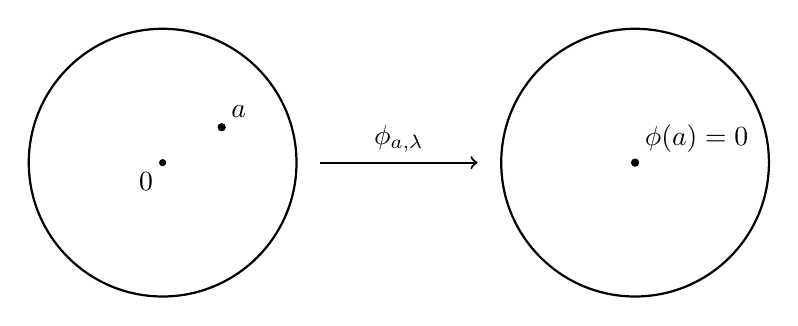
\begin{tikzpicture}[scale=1.0]
  \begin{scope}[xshift=-3.0cm]
    \draw[thick] (0,0) circle (1.7);
    \fill (0.75,0.45) circle (1.5pt) node[above right] {$a$};
    \fill (0,0) circle (1.3pt) node[below left] {$0$};
  \end{scope}
  \draw[->,thick] (-1.0,0)--(1.0,0) node[midway,above] {$\phi_{a,\lambda}$};
  \begin{scope}[xshift=3.0cm]
    \draw[thick] (0,0) circle (1.7);
    \fill (0,0) circle (1.5pt) node[above right] {$\phi(a)=0$};
  \end{scope}
\end{tikzpicture}
\caption{Every conformal automorphism of the disk is a Blaschke factor followed by a rotation: first send $a$ to $0$, then Schwarz's lemma forces the remaining normalized automorphism to be $z\mapsto\lambda z$.}
\label{fig:cp-iv-0080-schwarz-disk-automorphism}
\end{figure}
